\documentclass[journal]{IEEEtran}

% ===================
% Paquetes
% ===================
\usepackage[utf8]{inputenc}
\usepackage[T1]{fontenc}
\usepackage{lmodern}
\usepackage[spanish,es-noshorthands,es-tabla]{babel}
\usepackage{amsmath, amsfonts, amssymb}
\usepackage{graphicx}
\usepackage{cite}
\usepackage{xcolor}
\usepackage{array}
\usepackage{multirow}
\usepackage[hyphens]{url}
\usepackage{tikz}
\usetikzlibrary{babel,arrows.meta,positioning,fit,calc}
\usepackage{booktabs}
\usepackage{algorithm}
\usepackage[noend]{algorithmic}
% [H] fija tablas y algoritmos donde se escriben, entre su párrafo de
% introducción y su explicación.
\usepackage{float}
% Sin esto IEEEtran estira los espacios verticales para llenar la columna
% cuando un float [H] pasa a la siguiente, y quedan huecos grandes.
\raggedbottom
% Pseudocódigo en español.
\floatname{algorithm}{Algoritmo}
\renewcommand{\algorithmicif}{\textbf{si}}
\renewcommand{\algorithmicthen}{\textbf{entonces}}
\renewcommand{\algorithmicelse}{\textbf{si no}}
\renewcommand{\algorithmicelsif}{\algorithmicelse\ \algorithmicif}
\renewcommand{\algorithmicendif}{\textbf{fin si}}
\renewcommand{\algorithmicwhile}{\textbf{mientras}}
\renewcommand{\algorithmicdo}{\textbf{hacer}}
\renewcommand{\algorithmicendwhile}{\textbf{fin mientras}}
\renewcommand{\algorithmicrepeat}{\textbf{repetir}}
\renewcommand{\algorithmicuntil}{\textbf{hasta}}
\renewcommand{\algorithmiccomment}[1]{\hfill$\triangleright$~#1}
\usepackage[breaklinks=true,hidelinks]{hyperref}

% Bloque de "pendiente" bien visible en el PDF, para las secciones todavía
% sin escribir. Se reemplaza por contenido real antes de la entrega: el PDF
% entregado no debe contener ninguno (buscar "PENDIENTE" en main.log).
\newcommand{\pendiente}[1]{%
  \begin{quote}\small\color{black!60}%
  \textbf{[PENDIENTE --- #1]}
  \end{quote}%
  \typeout{PENDIENTE: #1}%
}

% Nombres de código en el texto.
\newcommand{\code}[1]{\texttt{#1}}

% IEEEtran pone "Index Terms" en inglés.
\renewcommand{\IEEEkeywordsname}{Palabras clave}

% ===================
% Título y autores
% ===================
\title{\LARGE Memoria Compartida Distribuida en Espacio de Usuario:\\
Contrato Expl\'icito, Coherencia por P\'agina y Evaluaci\'on Experimental}

\author{
    Isaac Francisco Moreno Fuentes,~\\
    Emmanuel Barrantes Vargas\\
    \thanks{Isaac Francisco Moreno Fuentes y Emmanuel Barrantes Vargas son estudiantes del curso MC 6004 Sistemas Operativos Avanzados, Tecnológico de Costa Rica, II semestre 2026.}
}

% ===================
% Documento
% ===================
\begin{document}
\maketitle

\begin{abstract}
Se implementa una memoria compartida distribuida en espacio de usuario: un
coordinador central y hasta cuatro procesos trabajadores comparten páginas de
4096 bytes por TCP, con un contrato explícito de adquirir y liberar en lugar de
fallos de página. El coordinador mantiene un directorio por página y aplica un
protocolo de un escritor o varios lectores con invalidación, de modo que nadie
lee datos obsoletos dentro de un intervalo adquirido. La corrección se
verifica con 192 casos automatizados, bajo AddressSanitizer,
UndefinedBehaviorSanitizer y ThreadSanitizer, y con un verificador que
reconstruye el estado desde el registro del coordinador. Los experimentos
muestran que volver a adquirir una página cuesta mensajes y no datos (de 22 a
274 mensajes con las mismas tres páginas transferidas), que poner contadores
independientes en una misma página multiplica el tiempo por 2,4 con cuatro
nodos sin cambiar el trabajo, y que repartir el cálculo de $\pi$ solo
compensa cuando el cómputo domina sobre el costo de coordinar.
\end{abstract}

\begin{IEEEkeywords}
memoria compartida distribuida, coherencia por página, exclusión mutua,
invalidación, falso compartimiento
\end{IEEEkeywords}

% ===================
% Secciones
% ===================
\section{Introducción}

El alcance, los experimentos y las preguntas de análisis de este
trabajo los fija el enunciado del proyecto~\cite{enunciado2026}.

\pendiente{el problema: varios procesos con espacios de direcciones separados que comparten páginas, y por qué un contrato explícito en vez de transparencia}

\pendiente{qué entrega este trabajo y cómo se organiza el resto del documento}


\section{Arquitectura y representación de la memoria}

\pendiente{los procesos: un coordinador de un solo hilo con poll() y de 1 a 4 trabajadores sobre TCP; diagrama}

\pendiente{la memoria: páginas de 4096 bytes, el marco local de cada trabajador y los datos confirmados del coordinador}

\pendiente{la API de libdsm: init, acquire, release, barrier, finalize, y qué promete cada una}


\section{Protocolo de coherencia y sincronización}

\pendiente{el estado por página en el coordinador: escritor, lectores, versión, cola FIFO y ronda de invalidación}

\pendiente{pseudocódigo de la adquisición y de la publicación}

\pendiente{los invariantes: un escritor o varios lectores, nunca ambos; el grant solo después de las confirmaciones; la versión crece de a uno}

\pendiente{la traza real: una transición READ a WRITE reconstruida del registro del coordinador, mostrando que el grant ocurre después de los ACK}


\section{Pruebas y verificación}

\pendiente{las 192 pruebas unitarias y de punta a punta, y qué cubre cada capa}

\pendiente{los sanitizadores y el detector de carreras}

\pendiente{el verificador que reconstruye su propio modelo del registro}

\pendiente{la inyección de fallos y lo que no se pudo verificar con la herramienta prevista}


\section{Evaluación experimental}

Las medidas salen de 160 corridas sobre 16 configuraciones, diez repeticiones
cada una, en un equipo con procesador Intel Core i7-1260P de 16 hilos, núcleo
Linux 6.18 bajo WSL2, GCC 13.3.0, glibc 2.39 y Python 3.12.3. Ninguna corrida
quedó descartada.

Antes de cada configuración se corre una repetición de calentamiento que se
descarta y queda declarada en el registro de la corrida. No es cosmética: la
primera corrida después de compilar llegó a medir la mitad que las siguientes
para el mismo trabajo, y promediarla habría metido el estado frío de la caché
dentro del resultado.

Las métricas de tráfico no las informa la aplicación: se derivan del registro
del coordinador. Los bytes incluyen los 32 de cabecera de cada trama, y la
página se cuenta una sola vez por transmisión. La desviación es la muestral.

\subsection{Localidad de lectura}

Un escritor publica una versión y un lector hace $M$ lecturas de la página
entera. Lo único que cambia es cuándo pide permiso: una sola adquisición para
las $M$ lecturas, o una por lectura. El trabajo local es idéntico en los dos
casos y está medido: las mismas $M$ verificaciones de 4096 bytes.

\begin{table*}[t]
\caption{Localidad de lectura con dos nodos y un lector.}
\label{tab:localidad}
\centering
\small
%% Generado por scripts/tablas_informe.py. No editar.
\begin{tabular}{@{}rlrrrrr@{}}
\toprule
lect. & permiso & tiempo (ms) & adq. & msjs. & bytes & págs. \\
\midrule
1 & una sola & $0,166 \pm 0,111$ & 1 & 22 & 13\,160 & 3 \\
1 & una por lectura & $0,139 \pm 0,026$ & 1 & 22 & 13\,160 & 3 \\
8 & una sola & $0,177 \pm 0,019$ & 1 & 22 & 13\,160 & 3 \\
8 & una por lectura & $1,157 \pm 0,172$ & 8 & 50 & 14\,168 & 3 \\
64 & una sola & $0,690 \pm 0,191$ & 1 & 22 & 13\,160 & 3 \\
64 & una por lectura & $8,056 \pm 0,679$ & 64 & 274 & 22\,232 & 3 \\
\bottomrule
\end{tabular}

\end{table*}

La última columna es el resultado: \textbf{tres páginas transferidas en los
seis casos}. Pedir permiso 64 veces en vez de una no mueve un solo byte de
datos extra en concepto de página; mueve mensajes. El tiempo pasa de 0,69 a
8,06~ms, 11,7 veces más, y los mensajes de 22 a 274.

La otra mitad del resultado es la fila que no cambia. Con una sola
adquisición, el costo en mensajes es 22 con 1, con 8 y con 64 lecturas: una
vez que el permiso está, leer es gratis en la red. La figura~\ref{fig:localidad}
muestra las dos cosas a la vez.

\begin{figure*}[t]
\centering
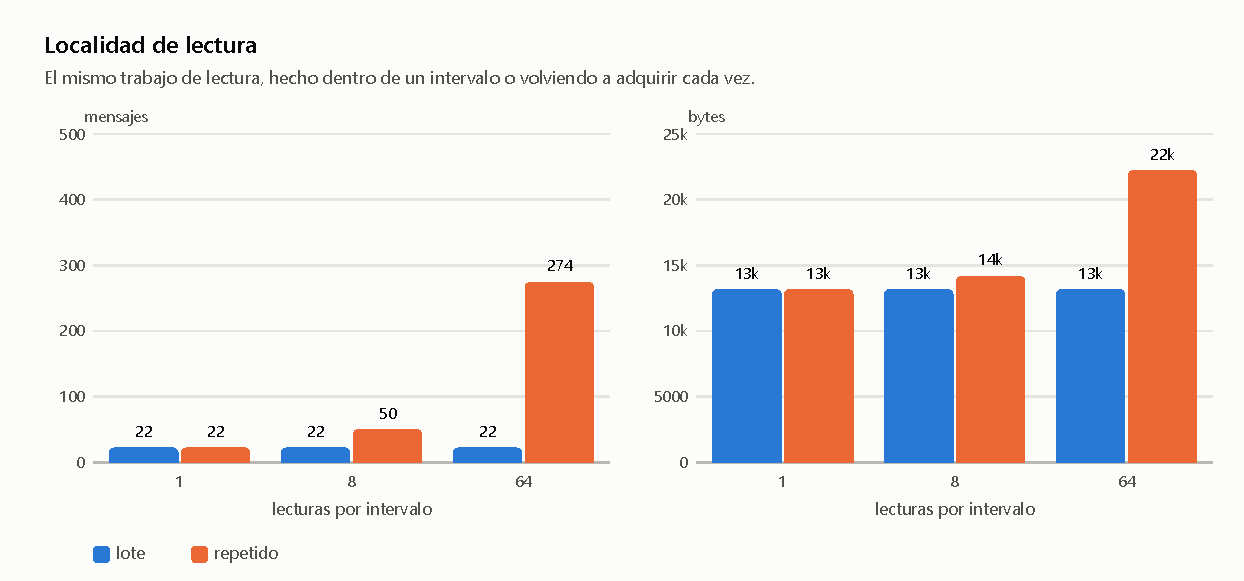
\includegraphics[width=0.86\textwidth]{figuras/fig1_localidad.pdf}
\caption{Mensajes y bytes según cuántas lecturas caben en una adquisición.}
\label{fig:localidad}
\end{figure*}

Los 13\,160 bytes de base no son del experimento: son el establecimiento de la
sesión, la publicación del escritor y las barreras. Por eso el crecimiento
relativo en bytes (1,7 veces) es mucho menor que el crecimiento en mensajes
(12,5 veces): lo que se agrega son tramas de 40 bytes, no páginas de 4096.

\subsection{Falso compartimiento}

Cada nodo incrementa \emph{su propio} contador 50 veces. Nadie lee el contador
de otro. Lo único que cambia entre los dos diseños es dónde viven los
contadores: todos en la página 0, u uno por página. El trabajo lógico es el
mismo y también está medido: 50 adquisiciones de escritura y 50 incrementos
por nodo en los dos diseños.

\begin{table*}[t]
\caption{Falso compartimiento con 50 rondas. El tiempo es el del nodo más
lento. Los bytes de coordinación son los de las barreras que ordenan las
rondas.}
\label{tab:fs}
\centering
\small
%% Generado por scripts/tablas_informe.py. No editar.
\begin{tabular}{@{}rlrrrrr@{}}
\toprule
$N$ & contadores & tiempo (ms) & inval. & b.\ coher. & págs. & b.\ coord. \\
\midrule
2 & misma página & $22,05 \pm 1,11$ & $96,0 \pm 2,1$ & 832\,640 & 198 & 8\,160 \\
2 & una por nodo & $14,05 \pm 1,09$ & 0 & 433\,280 & 102 & 8\,160 \\
4 & misma página & $42,87 \pm 3,23$ & $198,6 \pm 0,7$ & 1\,692\,736 & 403 & 16\,320 \\
4 & una por nodo & $17,86 \pm 0,75$ & 0 & 866\,560 & 204 & 16\,320 \\
\bottomrule
\end{tabular}

\end{table*}

Compartir la página cuesta 1,57 veces el tiempo con dos nodos y 2,40 con
cuatro, para un trabajo que la aplicación considera independiente. Las
invalidaciones pasan de cero a 96 y a 198,6 en promedio, los bytes de
coherencia casi se duplican y las páginas transferidas también.

\begin{figure*}[t]
\centering
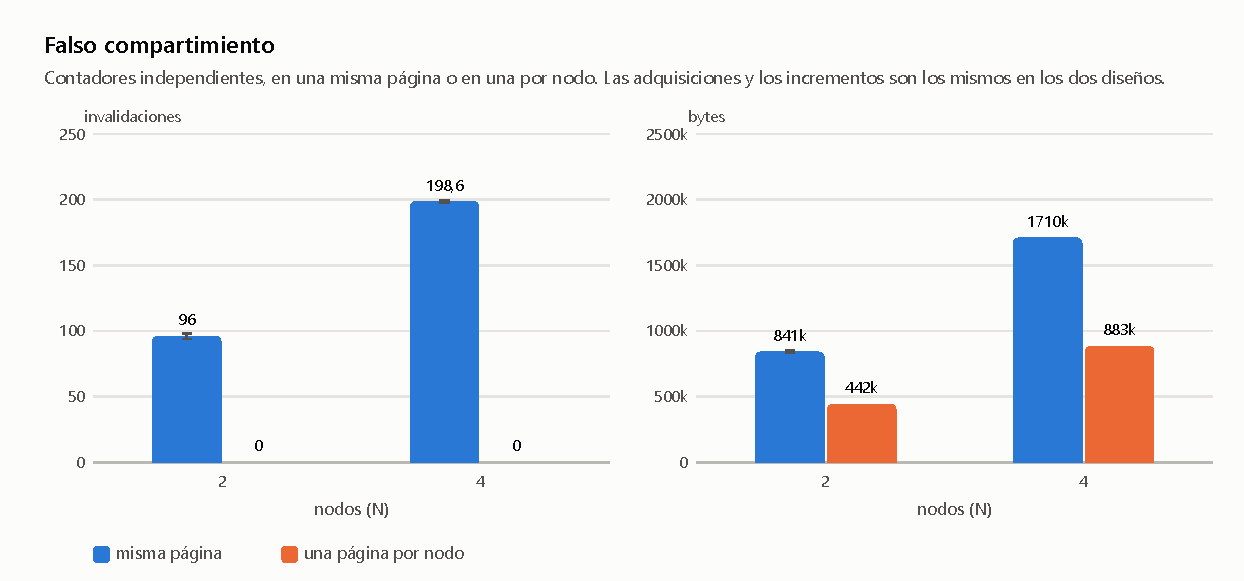
\includegraphics[width=0.86\textwidth]{figuras/fig2_false_sharing.pdf}
\caption{Invalidaciones y bytes según dónde viven contadores independientes.}
\label{fig:fs}
\end{figure*}

La columna que cierra el argumento es la última. Los bytes de coordinación son
\emph{idénticos} entre los dos diseños: 8\,160 con dos nodos y 16\,320 con
cuatro, en los dos casos. Las barreras que ordenan las rondas son las mismas,
así que no explican ninguna parte de la diferencia. Lo que cambia es
exclusivamente el tráfico de coherencia, y cambia porque la unidad de
coherencia es la página y no el dato.

\subsection{Costo de distribución}

La serie de Leibniz para $\pi$ con el mismo $T$ repartido entre $N$ nodos. Se
informan por separado el tiempo de la fase de cálculo y publicación, el total
de la sesión, y el de la serie secuencial de referencia que el nodo 0 calcula
para verificarse.

\begin{table*}[t]
\caption{Costo de distribución. La escala compara la fase de cálculo contra
la de un solo nodo con el mismo $T$.}
\label{tab:dist}
\centering
\small
%% Generado por scripts/tablas_informe.py. No editar.
\begin{tabular}{@{}rrrrrrr@{}}
\toprule
$T$ & $N$ & cálculo (ms) & total (ms) & secuencial (ms) & bytes & escala \\
\midrule
100\,003 & 1 & $0,47 \pm 0,06$ & $1,32 \pm 0,20$ & $0,22 \pm 0,03$ & 8\,776 & 1,00$\times$ \\
100\,003 & 2 & $0,61 \pm 0,23$ & $1,71 \pm 0,45$ & $0,22 \pm 0,05$ & 21\,568 & 0,77$\times$ \\
100\,003 & 4 & $0,89 \pm 0,14$ & $2,56 \pm 0,48$ & $0,20 \pm 0,00$ & 38\,960 & 0,53$\times$ \\
200\,000\,003 & 1 & $360,34 \pm 17,80$ & $712,01 \pm 33,35$ & $350,48 \pm 17,74$ & 8\,776 & 1,00$\times$ \\
200\,000\,003 & 2 & $209,56 \pm 19,40$ & $607,82 \pm 52,84$ & $396,88 \pm 37,34$ & 19\,520 & 1,72$\times$ \\
200\,000\,003 & 4 & $124,02 \pm 8,43$ & $567,71 \pm 17,30$ & $441,79 \pm 15,02$ & 37\,731 & 2,91$\times$ \\
\bottomrule
\end{tabular}

\end{table*}

Con $T$ grande la fase de cálculo escala 1,72 veces con dos nodos y 2,91 con
cuatro. El total baja mucho menos —de 712 a 568~ms— porque arrastra el
establecimiento de la sesión, las barreras y la serie de referencia, que no se
reparten entre nadie.

Con $T$ pequeño distribuir \emph{empeora} todo: el total sube de 1,32 a
2,56~ms al pasar de uno a cuatro nodos, y los bytes se multiplican por 4,4
mientras el cálculo tampoco baja. No hay nada que repartir, y lo único que se
mide es el costo de arrancar.

\begin{figure*}[t]
\centering
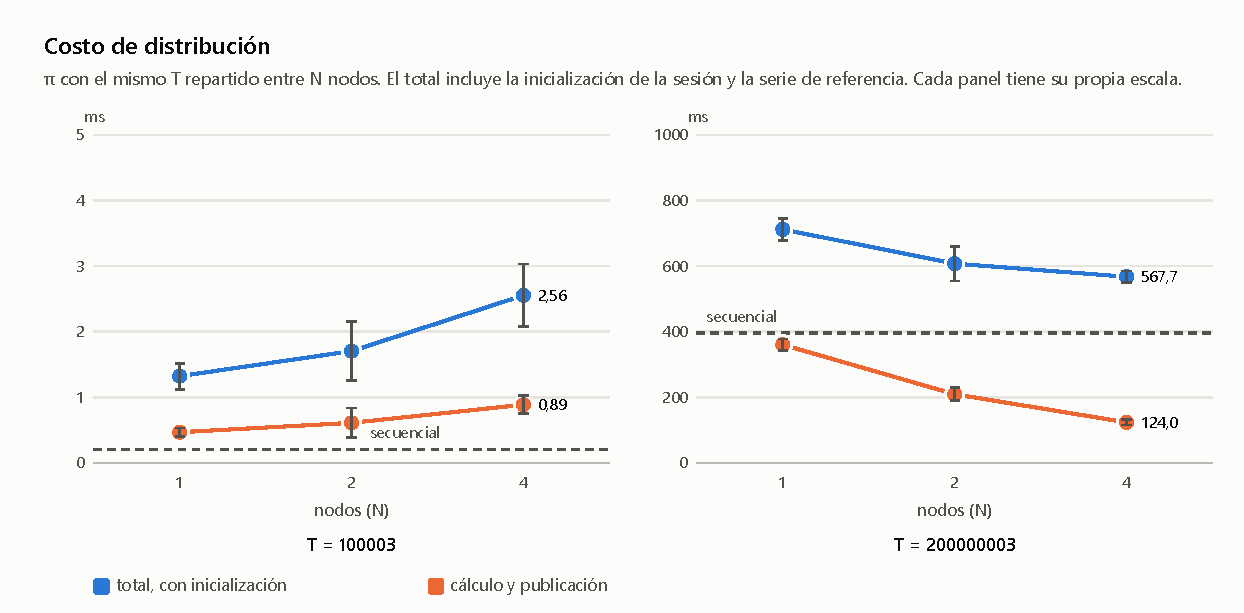
\includegraphics[width=0.86\textwidth]{figuras/fig3_distribucion.pdf}
\caption{Tiempo total y de la fase de cálculo contra la cantidad de nodos,
con la serie secuencial de referencia punteada. Cada panel tiene su escala.}
\label{fig:dist}
\end{figure*}

Hay una columna que no se puede leer como se leería en un banco de pruebas
limpio. El tiempo de la serie secuencial \emph{crece con $N$} —350~ms con un
nodo, 442 con cuatro— aunque el trabajo sea exactamente el mismo $T$. Esa
serie la calcula el nodo 0 mientras los demás procesos de la sesión están
vivos en la misma máquina, así que lo que mide de más es contención del
equipo, no del protocolo. La comparación que se sostiene es cálculo contra
cálculo, que es la que informa la columna de escala y la que dibuja la figura.

\section{Preguntas de análisis}

\subsection{Exclusión por página y operaciones sobre varias páginas}

La exclusión por página garantiza que, mientras un nodo tiene permiso de
escritura sobre una página, ningún otro la lee ni la escribe, y que lo que
publique será visible para quien adquiera después con una versión mayor. Es
una garantía \emph{por página y por intervalo}: vale entre el
\code{DSM\_acquire} y el \code{DSM\_release} de esa página.

No garantiza nada sobre una operación que abarque varias páginas. Si un nodo
adquiere la página 0, la modifica, la libera, y después adquiere la página 1,
otro nodo pudo haber escrito la página 1 en el medio —o haber leído la 0 ya
modificada y la 1 todavía vieja. Las dos escrituras son atómicas por separado
y el conjunto no lo es. El protocolo no ofrece ninguna forma de adquirir dos
páginas como una unidad, y adquirirlas de a una en orden fijo evita el
interbloqueo pero no produce atomicidad: solo evita que dos nodos se esperen
en círculo.

Una barrera final no corrige incrementos perdidos porque una barrera es una
afirmación sobre el \emph{tiempo}, no sobre el \emph{contenido}. Dice que
todos llegaron a este punto; no dice qué hizo cada uno antes de llegar. Si dos
nodos leyeron el valor 7, le sumaron uno y publicaron 8, el 8 es el valor
confirmado y la barrera posterior lo deja exactamente así. El incremento se
perdió en el momento en que el segundo nodo leyó antes de que el primero
publicara, y nada que ocurra después puede saber que ese 9 debió existir.

La forma de no perderlo es que la lectura y la escritura ocurran dentro del
mismo intervalo de escritura: adquirir en modo \code{WRITE}, leer, sumar y
liberar. Entonces el segundo nodo no puede leer hasta que el primero publicó,
y el protocolo lo impide por construcción, no por disciplina del programador.

\subsection{El coordinador central}

Para razonar sobre corrección, el coordinador central tiene una ventaja que
cuesta sobrevalorar: \emph{existe un único orden}. Todas las decisiones se
toman en un solo hilo, una por vez, sobre un estado que nadie más toca. Eso
convierte afirmaciones que serían difíciles —``ningún lector observó la página
mientras el escritor la tenía''— en propiedades de una máquina de estados que
se pueden comprobar después de cada transición y que se pueden leer en una
secuencia de filas numeradas.

También hace que la verificación sea posible desde afuera. El registro del
coordinador es la historia completa del sistema: no hay eventos que ocurrieran
en otro lado y que haya que correlacionar por reloj.

El costo está en el mismo lugar que la ventaja. El coordinador es un cuello de
botella de dos maneras. Por trabajo, todas las solicitudes pasan por un hilo,
aunque en este sistema ese hilo solo compara máscaras de bits y el límite real
está en la red. Y por tráfico: cada página publicada viaja al coordinador y
vuelve a salir hacia quien la pida, de modo que una transferencia entre dos
nodos cuesta dos veces la página en vez de una. Un protocolo con directorio
distribuido mandaría la página del dueño anterior al nuevo directamente.

Como punto único de fallo es total y está asumido: si el coordinador muere, la
sesión muere. No hay réplica del directorio ni de los datos confirmados, de
modo que no hay ningún estado del que otro proceso pudiera continuar. Los
trabajadores también son puntos únicos en un sentido más débil: la caída de
uno aborta la sesión, porque las barreras esperan a todos y una página que él
tuviera en escritura no tiene dueño que la publique.

\subsection{Tráfico cuando datos independientes comparten página}

El experimento de falso compartimiento responde esto con números. Con dos
nodos que incrementan contadores que nadie más mira, ponerlos en la misma
página sube el tráfico de coherencia de 433\,280 a 832\,640 bytes y las
páginas transferidas de 102 a 198; las invalidaciones pasan de cero a 96. Con
cuatro nodos, de cero a 198,6 invalidaciones y de 866\,560 a
1\,692\,736 bytes.
El trabajo de la aplicación es idéntico y los bytes de coordinación también:
lo único que cambió es un desplazamiento dentro de la memoria.

La razón es que el protocolo no sabe qué parte de la página le importa a
quién. Cuando un nodo pide escribir, se invalida la página completa en todos
los que tengan copia, aunque la zona que van a leer no se haya tocado. La
unidad de coherencia es la página y la granularidad del dato es irrelevante
para ella.

Replicar lecturas conviene cuando la página se lee mucho más de lo que se
escribe. Varios lectores coexisten sin costo entre ellos: cada uno paga la
transferencia una vez y después lee a velocidad de memoria mientras conserve
el permiso. El experimento de localidad lo muestra en la dirección contraria:
el costo no está en leer sino en volver a pedir permiso.

Deja de convenir en cuanto aparece una escritura, y el costo que agrega no es
el de la escritura sino el de las copias. Escribir una página que nadie más
tiene es un mensaje y una transferencia. Escribir una que tienen otros tres
cuesta además tres invalidaciones, tres confirmaciones, y la próxima lectura
de cada uno vuelve a traer los 4096 bytes. El costo de escribir crece con la
cantidad de copias, no con el tamaño del dato que se escribió.

\subsection{Los costos que la interfaz oculta}

La interfaz de memoria compartida oculta que cada acceso puede ser una
conversación. \code{DSM\_acquire} parece una operación local y puede costar
una solicitud, una ronda de invalidaciones con sus confirmaciones, una espera
en cola detrás de otros nodos y una transferencia de 4096 bytes. El puntero
que devuelve se usa con instrucciones comunes, y esa es exactamente la
apariencia que esconde el costo.

También oculta el momento. El dato que se lee es el de la última publicación,
que puede ser de hace un microsegundo o de hace un minuto; nada en la interfaz
distingue esos dos casos. Y oculta la granularidad: el programador declara
variables, el protocolo mueve páginas, y el falso compartimiento vive
enteramente en la distancia entre esas dos unidades.

Nuestro contrato mitiga esto no por ser más barato, sino por ser explícito. El
costo sigue estando, pero aparece donde el programador escribió una llamada.
Eso es lo que permite medirlo por intervalo y atribuirlo a una línea de
código.

Recuperar la transparencia por fallos de página —que la aplicación use
punteros comunes sin pedir permiso— requeriría bastante más que interceptar la
señal. Haría falta delimitar la región de memoria que es DSM y protegerla con
\code{mprotect}, para que el acceso a una página sin permiso produzca un
fallo. Habría que distinguir ese fallo de un \code{SIGSEGV} genuino de la
aplicación y reenviar los ajenos al manejador que correspondiera, porque
tragárselos convertiría un error del programa en un cuelgue. El manejador
corre en contexto de señal, donde casi nada es seguro de llamar: no se puede
abrir un socket, ni esperar una respuesta, ni tomar un cerrojo que el hilo
interrumpido pudiera tener. La comunicación tendría que delegarse a un hilo
aparte, con el manejador limitado a despertarlo y esperar, usando únicamente
operaciones permitidas en ese contexto.

Después quedaría el problema que el permiso de página no resuelve: con
\code{mprotect} se detecta el primer acceso de escritura, pero no se sabe
\emph{qué} se escribió sin comparar la página contra una copia previa, ni
cuándo la región crítica terminó, porque ya nadie llama a \code{release}. Eso
obliga a elegir un modelo de consistencia relajado y un punto de
sincronización explícito de todas formas —una barrera, un cerrojo— con lo
cual parte de la transparencia que se buscaba vuelve a la interfaz por otra
puerta.

\section{Relación con la DSM transparente}

\pendiente{la DSM transparente: ilusión de memoria unificada, mapeo por fallos de página sobre la MMU, y que oculta la red pero no su costo}

\pendiente{en qué se diferencia nuestro contrato acquire/release: el costo es visible porque el programador lo pide}

\pendiente{qué NO se afirma: no es consistencia secuencial general ni TreadMarks}


\section{Decisiones de diseño}

\pendiente{las decisiones que explican por qué el código quedó así, contadas sin códigos ni referencias a la bitácora}


\section{Límites de alcance}

El sistema está pensado para que una sesión termine bien o termine; no para
que sobreviva a la pérdida de un participante. Conviene decir con precisión
qué significa eso, porque es la diferencia entre una limitación conocida y una
promesa incumplida.

\emph{No hay reconexión.} Un nodo que pierde la conexión no vuelve. No existe
un procedimiento para que se reincorpore con su estado, ni un identificador
que le permita reclamar lo que tenía. El conjunto de participantes se fija al
abrir la sesión y solo puede reducirse.

\emph{No hay recuperación de escrituras no publicadas.} Lo que un nodo escribió
en su marco local y todavía no liberó existe únicamente en su memoria. Si el
proceso muere con un permiso de escritura tomado, ese trabajo se pierde entero
y no hay forma de reconstruirlo: el coordinador nunca lo vio.

\emph{No hay persistencia.} Los datos confirmados viven en la memoria del
coordinador. Cuando la sesión termina, el contenido de las páginas desaparece.
No hay volcado a disco, ni bitácora de escrituras, ni manera de retomar una
sesión anterior.

\emph{No hay tolerancia a particiones.} Una red que se divide no produce dos
mitades que sigan trabajando: produce nodos que dejan de alcanzar al
coordinador y que, por lo tanto, dejan de poder adquirir nada. No hay quórum,
ni elección, ni reconciliación posterior.

Lo que sí hay es un corte limpio, y se distingue según cómo ocurra la pérdida.

Si el coordinador recibe una señal de terminación, avisa: le encola un error
de sesión abortada a cada nodo vivo, vacía las salidas con un tope, y recién
entonces cierra. Cada trabajador recibe un código que dice qué pasó, en vez de
descubrirlo cuando una lectura falla.

Si el coordinador muere sin ejecutar una instrucción más, no hay aviso posible
y tampoco hace falta inventarlo: el núcleo cierra sus sockets, el cierre llega
a cada trabajador y todos lo ven en el acto. Ésa es toda la garantía que se
puede dar en ese caso, y alcanza para que nadie quede esperando.

Del lado del trabajador, un error de sesión es terminal. La biblioteca rechaza
localmente todo lo que puede detectar antes de enviarlo —página fuera de
rango, modo inválido, adquisición anidada—, así que un error que llega desde
el coordinador a un trabajador correcto solo puede venir de un defecto. Seguir
operando sobre un estado que no se entiende es peor que terminar: lo que se
corrompe es la memoria compartida, y el síntoma aparecería lejos de la causa.

Hay además tres límites de tamaño que no son fallas sino decisiones fijadas en
tiempo de compilación: la página mide 4096 bytes, la sesión admite a lo sumo
cuatro nodos, y la cantidad de páginas se fija al arrancar y no cambia. El
primero es el que más se nota en los resultados, porque es la unidad de
coherencia y por lo tanto el tamaño del falso compartimiento. Comparar otro
tamaño de página era una de las ampliaciones posibles del enunciado y no se
hizo; el código la admite —el tamaño es una constante de compilación y no hay
ningún valor literal que dependa de ella— pero las pruebas sí dan por sentado
el tamaño actual, de modo que una construcción con otro valor sirve para medir
y no para correr la suite.

\section{Conclusiones}

\pendiente{qué quedó demostrado y qué seguiría}


\section{Declaración de transparencia}

\pendiente{uso de herramientas de IA y material reutilizado del Proyecto 2, con su procedencia y licencia}


\section*{Entrega}

\begin{itemize}
\item \textbf{Repositorio:} \url{https://github.com/ebarrantes07/SOA-P3-GrupoIE}
\item \textbf{Etiqueta:} \texttt{p3-entrega}
\end{itemize}

El identificador completo del commit etiquetado se registra en el comprobante
de entrega y no en este documento, porque el informe forma parte de ese commit.
La trazabilidad del trabajo está en el README del repositorio.


% ===================
% Referencias
% ===================
\bibliographystyle{IEEEtran}
\bibliography{referencias}

\end{document}
